\chapter{Result From Flight Data}\label{ch:FlightResult}

This chapter discussed the result of applying the proposed algorithm
on realistic aerial video and navigation data. Firstly, a piece of
video of 400 frames were processed by the CC\_EKF\_SLAM algorithm. The
convergence, accuracy and consistency of the result were analyzed
against ground truth, and described in section
\ref{sec:flight-converge}-\ref{sec:flight-consistency}. While
analyzing pure natural scene video where no man-made object can be
seen, it was found that landmarks correspondence between the
estimated and ground truth was difficult due to the
similarity in apperance of the landmark. Therefore, an another video
where landmarks can be manually and distinctively matched was
processed, and result was summarized in section \ref{sec:flight-manual}.

\section{Convergence}\label{sec:flight-converge}
When a landmark was added to the filter, the landmark initialization
point were initialized to the zero which is the origin of the camera
centric coordinate. $\phi$ and $\theta$ were calculated directly from
the feature position on image plane, had relatively high accuracy, and
should stay relatively constant. The only parameter that experienced
a converging process was the inverse depth $\rho$, which were
initialized to 0.1 for all landmarks.

Figure \ref{fltfig:1} shows the $1/\rho$ plot for the entire 400
frames. Landmark ID was shown on the right side of the plot for the
landmarks that were not converging. The depth estimates went through
rapid changes for several frames after initialization. Within
approximate 20 frames, most inverse depth estimates settled to stable
values. Sharp spike in the middle of the tracking is due to new
landmarks added into the filter. The estimated landmarks distances
ranged from 400 meters to about 1200 meters, confirming the
algorithm's capability for estimating landmarks at great distance. On
the other hands, some landmarks took a long time to settle, while some
other never settled and drift away as tracking continued, such as
landmark 32, 13, and 53. 
% An outlier filter should be in place to get rid of the poor features
% (future work).

\begin{figure}[h]
\centering
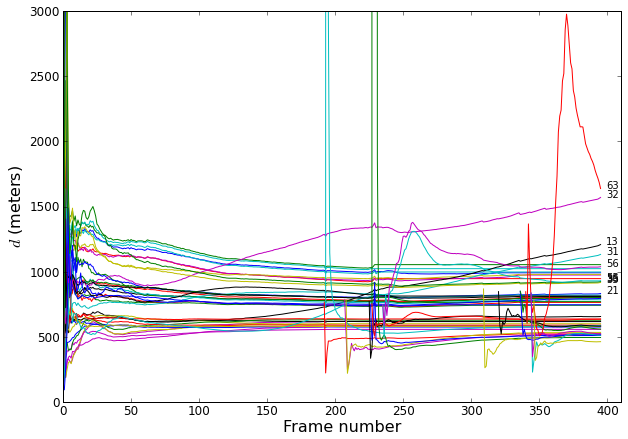
\includegraphics[width=12cm, keepaspectratio=true]{./Figures/fltfig/cut1/Figure10.png}
\caption{Inverse Depth Convergence}
\label{fltfig:1}
\end{figure}

The non-converging landmarks were those located at the edge of a hill
where objects with big difference in distance meet in the image. As an
example, visual pattern of landmark 13 at frame 50, 100, 150, 200,
250, 300, 350 and 398 were shown in figure \ref{fltfig:1_1}. It showed
that the initial visual pattern for landmark 13 was detected at the
edge of a hill top. As frame number advanced, the view the camera
became different. The pattern comparison in tracking algorithm
normally allows for a small error at each iteration to tolerate the
slight view change of the camera. This error accumulated slowly and
eventually caused the tracked target to become a pattern located at a
different location, which explained the slow drift in depth estimate.
To increase the reliability of the estimates, it is necessary to add
procedure into the algorithm to detect and handle such behavior.

\begin{figure}[h]
\centering
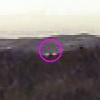
\includegraphics[width=3cm,
keepaspectratio=true]{./Figures/fltfig/cut1/features/uav2_cut1_050_fID13.jpg}
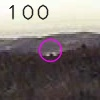
\includegraphics[width=3cm,
keepaspectratio=true]{./Figures/fltfig/cut1/features/uav2_cut1_100_fID13.jpg}
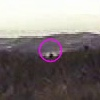
\includegraphics[width=3cm,
keepaspectratio=true]{./Figures/fltfig/cut1/features/uav2_cut1_150_fID13.jpg}
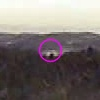
\includegraphics[width=3cm,
keepaspectratio=true]{./Figures/fltfig/cut1/features/uav2_cut1_200_fID13.jpg}
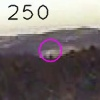
\includegraphics[width=3cm,
keepaspectratio=true]{./Figures/fltfig/cut1/features/uav2_cut1_250_fID13.jpg}
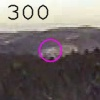
\includegraphics[width=3cm,
keepaspectratio=true]{./Figures/fltfig/cut1/features/uav2_cut1_300_fID13.jpg}
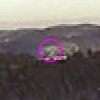
\includegraphics[width=3cm,
keepaspectratio=true]{./Figures/fltfig/cut1/features/uav2_cut1_350_fID13.jpg}
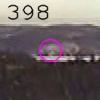
\includegraphics[width=3cm,
keepaspectratio=true]{./Figures/fltfig/cut1/features/uav2_cut1_398_fID13.jpg}
\caption{Feature 13 at frame 50, 100, 150, 200, 250, 300, 350, and 398}
\label{fltfig:1_1}
\end{figure}

When landmarks were initialized, the initialization coordinate $[x_i,
y_i, z_i]$, and the deviation-elevation angle pair $[\varphi, \theta]$
did not go through a slow converging stage. Ideally, the parameters
should stay at a relatively fixed value. As these parameters were used
with the inverse depth to calculate landmark coordinates on image
plane and received every iteration, their values were affected by the
inverse depth, and varied at each iteration. The plots in figure
\ref{fltfig:2} showed the variation of these parameters over the
entire processed frames.

First column of the plots showed landmark initialization coordinates
with the initial value subtracted. All landmarks that were initialized
at $1^{st}$ image frame had stable value with little variation.
Landmarks that were added at later image frames showed significant
drift from their initial value. This is a direct result of the filter
correction process. When a new landmark were added to the filter, it
had not established correlation with all the other landmarks and the
world frame parameters, which caused its correction on initialization
point slightly different than all the existing features and the world
frame position. As a future improvement, it is reasonable for the
newly added landmark to inherent the cross-correlation on the
initialization coordinates from a landmark close to it. elements.

Second and third columns showed the landmarks' $\varphi$ and $\theta$
parameters with their initial value or mean value subtracted. For all
landmarks, whether initialized at first image frame, or later frames,
these angle estimates all diverged slightly from the initial values.
This is not surprising since the initial depths of the landmarks were
unknown. To compensate for the incorrect depth, filter must change
$\varphi$ and $\theta$ estimates slightly to arrive at a predicted
measurements that agreed with the actual measurements. Secondly, the
SUAS rotation motion contributes to the variation pattern of $\varphi$
and $\theta$ estimates. \colorbox{yellow}{$\varphi$ is highly correlated with
  the Z rotation, and $\theta$ is correlated to the X
  rotation.(Verification required).} This behavior
suggested that the algorithm might be highly sensitive to aircraft
rotational motion.
% doesn't make sense. By definition, X rotation should have bigger
% impact on varphi, Z rotation has bigger impact on theta

\begin{figure}[h]
\centering
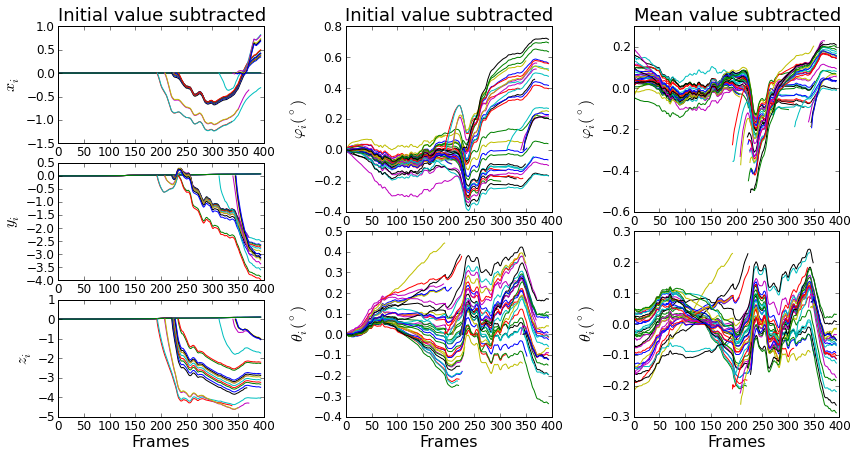
\includegraphics[width=14cm, keepaspectratio=true]
{./Figures/fltfig/cut1/Figure20.png}
\caption{Landmark parameters tracking}
\label{fltfig:2}
\end{figure}
% THIS WAS THE OLD TEXT, MAY NOT BE TRUE. 
% On the other hand, features
% mapping is not affected too much by the error in localization. Because
% their parameters are transformed in each iteration to the new camera
% frame using the estimated SUAS motion which carries the error. As long
% as their parameters are updated together with the estimated motion on
% that iteration, and transformed back to the world frame using the same
% estimated motion, the final result of features location in world frame
% is unaffected by the error in the SUAS localization. However, for
% feature removed from the filter, their parameters are no longer
% updated, therefore revealing the error in SUAS localization.
\FloatBarrier

\section{Accuracy}\label{sec:flight-accuracy}
\subsection{SUAS Localization}

The SUAS location and orientation were verified in UTM coordinate with
initial position removed. Ground truth data comes from the GPS for
position, and magnetometer for orientation. The GPS positioning can
generally achieve 7.8 meters in accuracy \cite{_gps_????}. For
orientation, accuracy on the GS-111m datasheet specified $0.1^{\circ}$
for roll and pitch, and $0.5^{\circ}$ for heading. Figure
\ref{fltfig:6} shows the estimated SUAS position and orientation,
ground truth data, and the error. From the comparison, X position
error reached a maximum of 20 meters, while error on Y and Z are
bigger, reaching 50 meters and 30 meters respectively. The position
error increases as the frame number grew bigger. For orientation, the
estimated value agrees with the ground truth pattern, with maximum
error within 0.02 rad or $1.15^{\circ}$. Although the error of pitch
is biased to the negative side, and error of heading is biased to the
positive side, there was no clear sign of diverging within the 400
frames processed.

\begin{figure}[h]
\centering
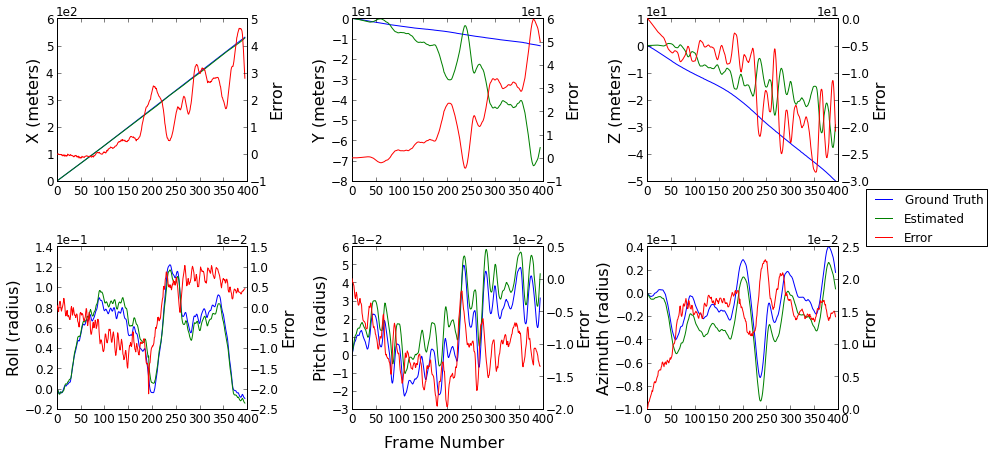
\includegraphics[width=12cm, keepaspectratio=true]
{./Figures/fltfig/cut1/Figure30.png}
\caption{SUAS position and orientation}
\label{fltfig:6}
\end{figure}
\FloatBarrier
\subsection{Features Mapping}\label{sec:accuracy_features}

The ground truth data came from digital terrain map (DEM) can be
downloaded from CGIAR-CSI website \cite{_cgiar-csi_????}. Making data
correspondence with the estimated feature is non-trivial for natural
scene where it lacks of distinguishable landmark such as building corners or
other man-made objects. From the experience of analyzing simulation
data (chapter \ref{ch:simulation}), the initialized feature deviation
and elevation angle $\phi$ and $\theta$ agrees very well to the ground
truth value. In addition, feature initialization position is set to
$[0, 0, 0]$ in camera frame, therefore carries no error. Therefore, the
following procedure are used the find the corresponding ground truth
location for any estimated feature.

\begin{enumerate}
  \item The frame number at which feature was initialized was
  identified, and ground truth position and orientation of the SUAS at
  that frame was recorded.
  \item Create a reference frame on DEM at the feature initialization point.
  \item Convert the feature deviation $\theta$ and elevation $\phi$
  angle to UTM frame. (These angles were recorded in camera frame)
  \item Create a vertical plane using $\theta$ and slice the DEM to
  form a 1D elevation plot (Example: figure \ref{fltfig:7} blue line)
  \item Create a line using $\phi$ and intersect the 1D elevation plot
  (Figure \ref{fltfig:7} green line). 
  \item The $1^{st}$ intersection point is used as ground truth
  feature location.
\end{enumerate}

\begin{figure}[h]
\centering
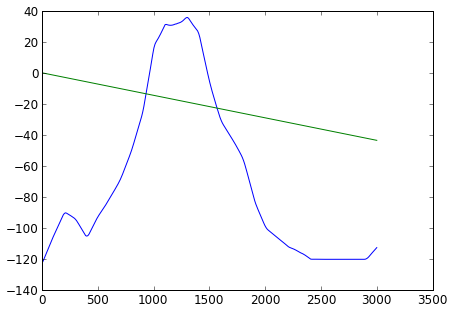
\includegraphics[width=12cm, keepaspectratio=true]
{./Figures/fltfig/cut1/intersect0_0.png}
\caption{Finding ground truth feature position on DEM}
\label{fltfig:7}
\end{figure}

Feature locations are compared in world frame for the ease of
corresponding the estimated features the video by eye. The error
convergence is plotted in figure \ref{fltfig:8}. X component (along
which axis the SUAS is traveling) of feature position converge to zero
in general with maximum error less than 120m for the converged
features. Y component shows a clear offset for features not
initialized at first frame. This behavior is similar to what's seen in
the simulation analysis \ref{sec:featureMotion} where offset in
features position estimates are caused by drift in SUAS localization
estimation. Z component does not show such offset.

\begin{figure}[h]
\centering
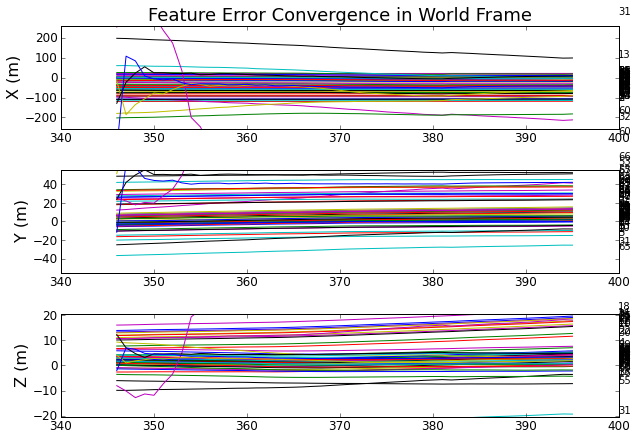
\includegraphics[width=10cm, keepaspectratio=true]
{./Figures/fltfig/cut1/Figure50.png}
\caption{Feature position error convergence}
\label{fltfig:8}
\end{figure}

Plotting the estimated and ground truth features position vs feature
initialization sequence reveals more detail on the feature position
error. Figure \ref{fltfig:9} plots the estimated and ground truth
feature positions on the left, and error on the right. First for X
component, the biggest error occur on feature number 65 which is
initialized fairly late in the sequence, and has not converged
properly. On Y axis, the position plot also shows feature number
higher than 40 carries an offset error. In addition, the average error
is increasing as feature number gets bigger, which indicate the
further the feature initialization point is from the world origin, the
bigger this offset error will be. When plotting the feature error vs.
feature's ground truth postion (figure \ref{fltfig:err_vs_gtpos}), it
shows that the biggest Z axis error happens to the feature located
closest to the camera and with the biggest Z ground truth position,
which is the very bottom region of the image frame. This position
suggested that the Z axis error might be related to the lens
distortion that was not taken into account in this algorithm.

\begin{figure}[h]
\centering
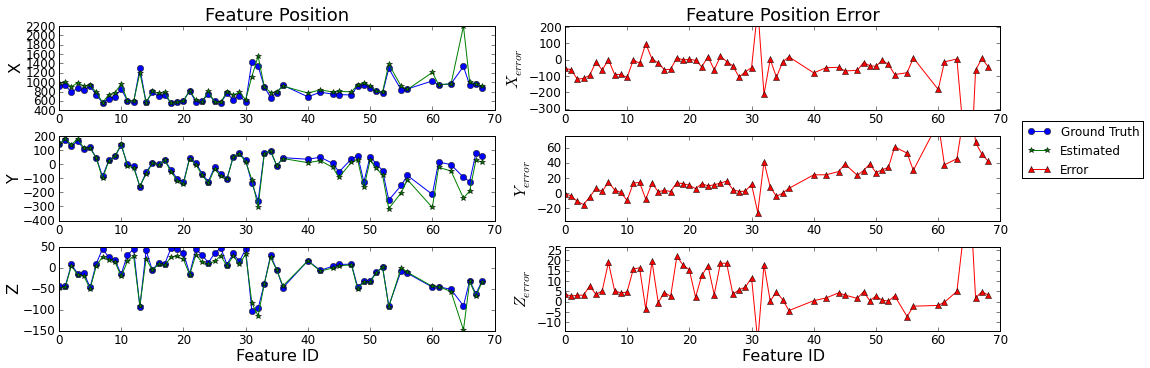
\includegraphics[width=14cm, keepaspectratio=true]
{./Figures/fltfig/cut1/Figure60.png}
\caption{Feature position error plotted vs initialization sequence. }
\label{fltfig:9}
\end{figure}

\begin{figure}[h]
\centering
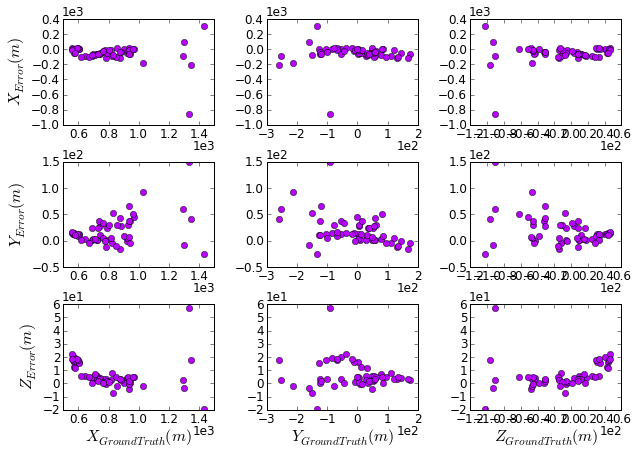
\includegraphics[width=14cm, keepaspectratio=true]
{./Figures/fltfig/cut1/Figure80.png}
\caption{Feature position error plotted vs. ground truth position. }
\label{fltfig:err_vs_gtpos}
\end{figure}

Using the estimated feature position, a terrain map can be generated.
Figure \ref{fltfig:10} shows the terrain map generated from the
feature position analyzed above. On the right, the ground truth DEM is
also shown for comparison. 

\begin{figure}[h]
\centering
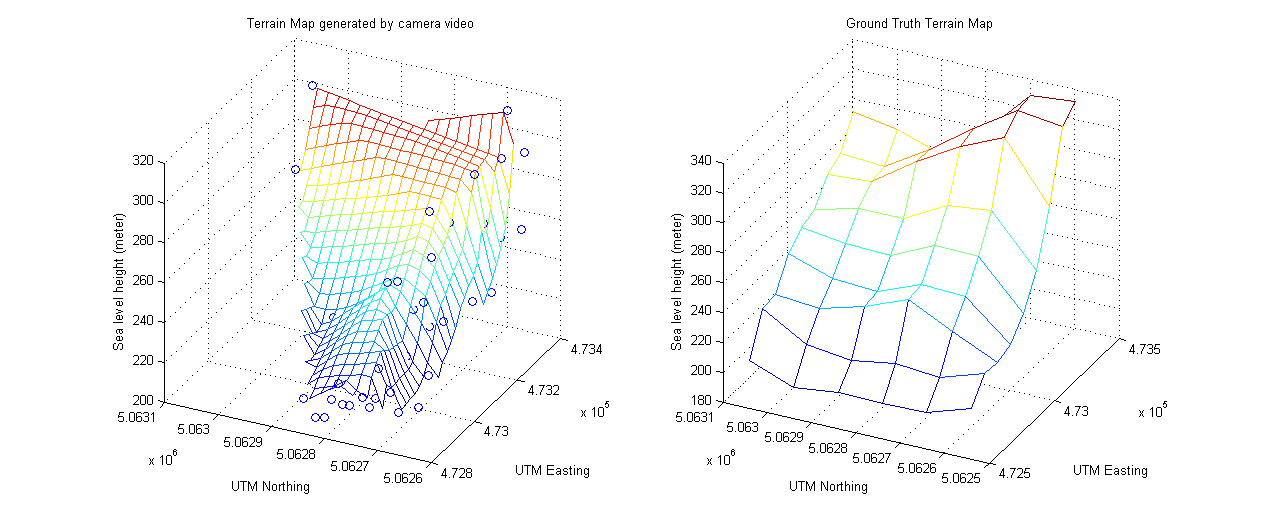
\includegraphics[width=14cm, keepaspectratio=true]
{./Figures/fltfig/cut1/terrain/terrain_map_cmp.png}
\caption{Terrain map. Left: estimated, right: ground truth }
\label{fltfig:10}
\end{figure}
\FloatBarrier

\section{Consistency Analysis}\label{sec:flight-consistency}
A EKF system becomes inconsistent when the variance of state vector
element becomes too small and forbid an effective update. In addition,
the uncertainty of the world frame should increase as the camera frame
moves away from it. To examine the consistency of the CC\_EKF\_SLAM
algorithm, the variance of world frame parameters and camera motions
are plotted in \ref{fltfig:120}, and variance of features parameters
are plotted in figure \ref{fltfig:3}. The variance of world frame
position increases with iterations at the beginning, and after frame
100, $\sigma^2_{O_Y}$ and $\sigma^2_{O_Z}$ converged. This is
likely due to the little variation on the Y and Z translation of the
SUAS. On the other hand, camera rotation and world frame orientation
variance has similar pattern and amplitude. The X component decreases
with iterations. Y and Z components fluctuate around a fixed value and
remain below 1.5e-5$^\circ$. Although world frame variance remains fixed
at prediction, camera rotations had a 1$^\circ$ noise added at
prediction (as indicated by the GS-111m specification
\cite{_athena_????}). The update process reduced the noise of camera
rotation significantly and resulted in a variance estimates much lower
than the specification. Affected by the camera rotation variance,
features parameter $\varphi$ and $\theta$ also carries a very small
variance.

% does increasing measurement variance increases parameter variance? 

\begin{figure}[h]
\centering
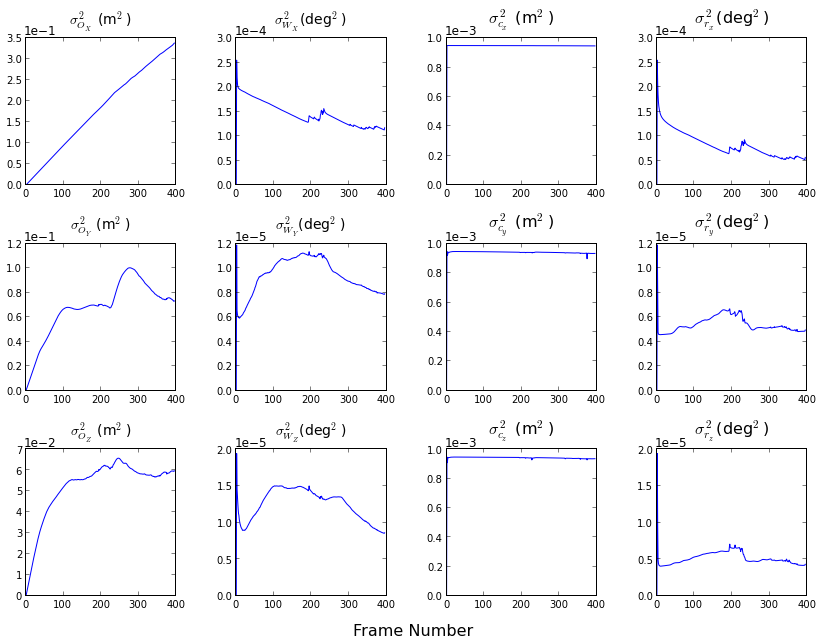
\includegraphics[width=14cm, keepaspectratio=true]
{./Figures/fltfig/cut1/Figure120.png}
\caption{Variance of world frame parameters and camera motion}
\label{fltfig:120}
\end{figure}


\begin{figure}[h]
\centering
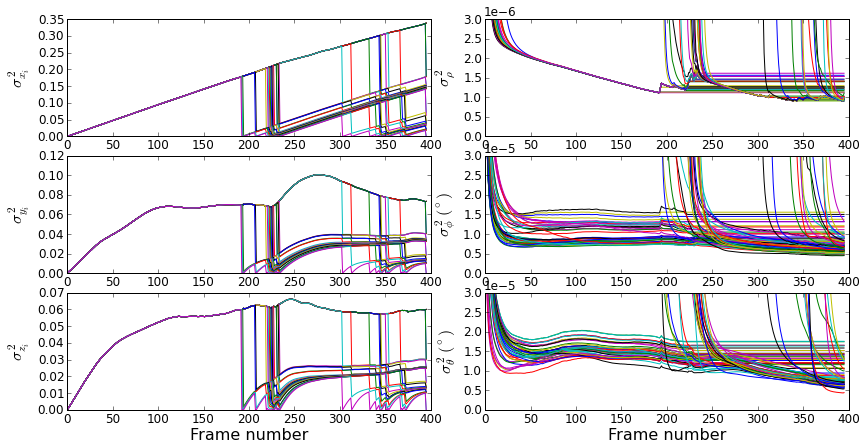
\includegraphics[width=14cm, keepaspectratio=true]
{./Figures/fltfig/cut1/Figure40.png}
\caption{Variance of features parameters}
\label{fltfig:3}
\end{figure}
\FloatBarrier

To see how variance affect the correction the filtered made on the
state vector, the correction applied in camera frame were plotted in
figure \ref{fltfig:4}. The $1^{st}$ column shows the correction on
world frame position. The $2^{nd}$ column shows the correction on
feature initialization coordinate. The $3^{rd}$ column shows the
correction on features parameters $\rho$, $\varphi$ and $\theta$. It
can be observed that in general the correction amount agrees with the
variance that bigger variance results in more correction, except for
the world frame Y and Z position and camera Y and Z motion. These
parameters receives more correction as tracking progress despite their
variance stabilized or even decreased. Secondly, there is a strong
correlation between the feature initialization position and the world
frame position on Y and Z axis. At the same time, world frame and
feature initialization is inversly correlated to the camera motion on
Y and Z axis. Thirdly, the camera parameter corrections shows an
obvious trend only on Y and Z motion. Due to these correlation, the
main contributor for all the drift in SUAS position and offset in
feature mapping should be coming from the camera motion correction on
Y and Z axis. On the other hand, the big correction on these
parameters could be caused by the small variance in the camera
rotation variance. If not enough correction can be made into the
camera rotation and $\varphi$ and $\theta$ angles, the algorithm has
to compensate that by making more adjustment in the camera motion on Y
and Z. This issue requires further investigation, and will be analyze as a
future work.

\begin{figure}[h]
\centering
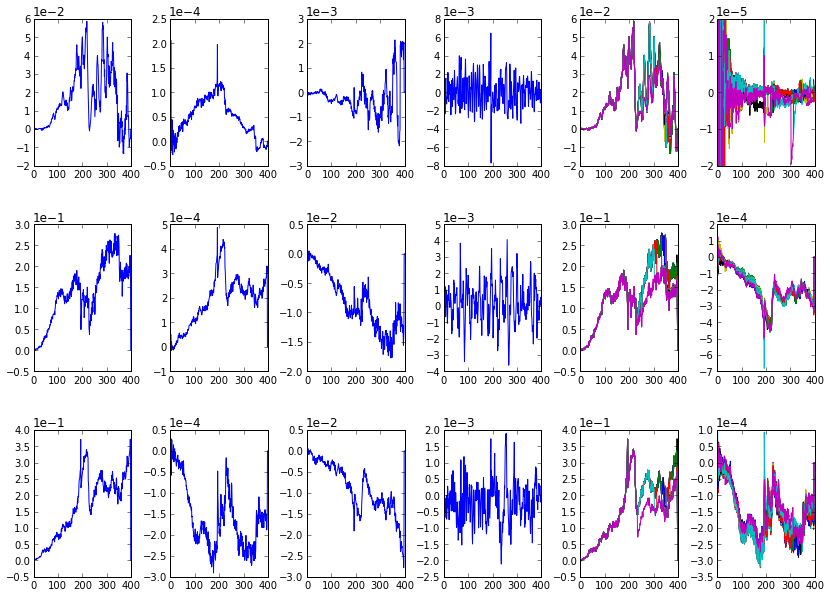
\includegraphics[width=12cm, keepaspectratio=true]
{./Figures/fltfig/cut1/Figure112.png}
\caption{State Vector Corrections}
\label{fltfig:4}
\end{figure}

\FloatBarrier

\section{Compare to Visually Corresponded Feature}
\label{sec:flight-manual}
Due to the difficulty of corresponding feature extracted from video to the
actual data on DEM, a second piece of video was processed with
man-made structure in the scene so that feature correspondence can be
made manually. Figure \ref{fltfig:11} shows a zoomed in view of the
features extracted by the CC\_EKF\_SLAM. All features are located at
the bottom left corner of the image. Figure \ref{fltfig:12} shows the
common features found manually on the satalite image on Google Earth
\cite{_google_????}.

\begin{figure}[h]
\centering
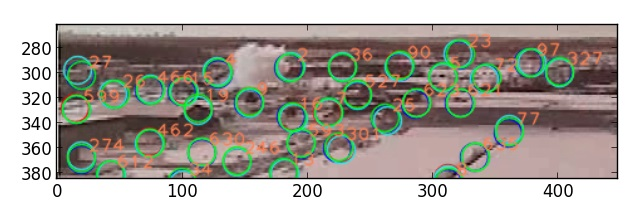
\includegraphics[width=10cm, keepaspectratio=true]
{./Figures/fltfig/airport/frame398_features.jpg}
\caption{Feature identified by algorithm }
\label{fltfig:11}
\end{figure}

\begin{figure}[h]
\centering
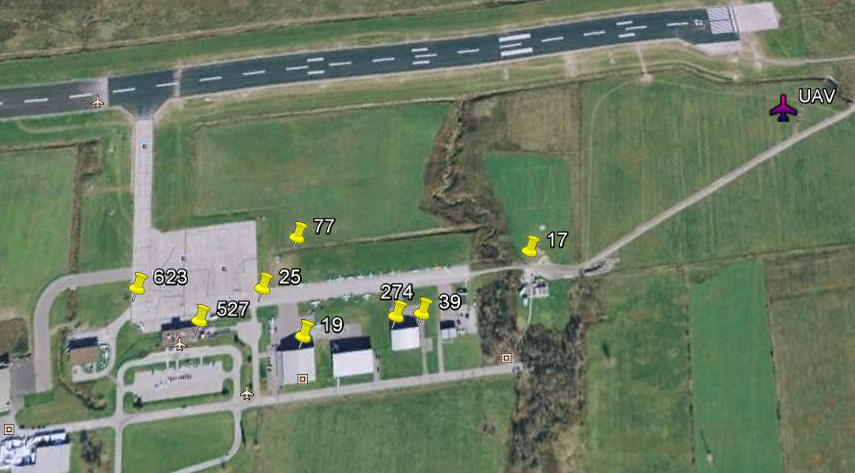
\includegraphics[width=13cm, keepaspectratio=true]
{./Figures/fltfig/airport/uav_and_identified_landmark.png}
\caption{Common features idetified manually on Google Earth }
\label{fltfig:12}
\end{figure}
\FloatBarrier

The SUAS position and orientation were compared to onboard GPS and INS
recording, and the result are plotted in figure \ref{fltfig:13} and
figure \ref{fltfig:14}. Similar to the natual scene video, SUAS
location is more accurate on X, and shows more drift on Y and Z
coordinate. The drift become significant when frame number exceeds
200. However, with the SUAS decending, drift on Z is less than the
amount when it ascended. For orientation error, roll and pitch error
oscillate around zero, but azimuth error drift away as frame number
increases.

\begin{figure}[h]
\centering
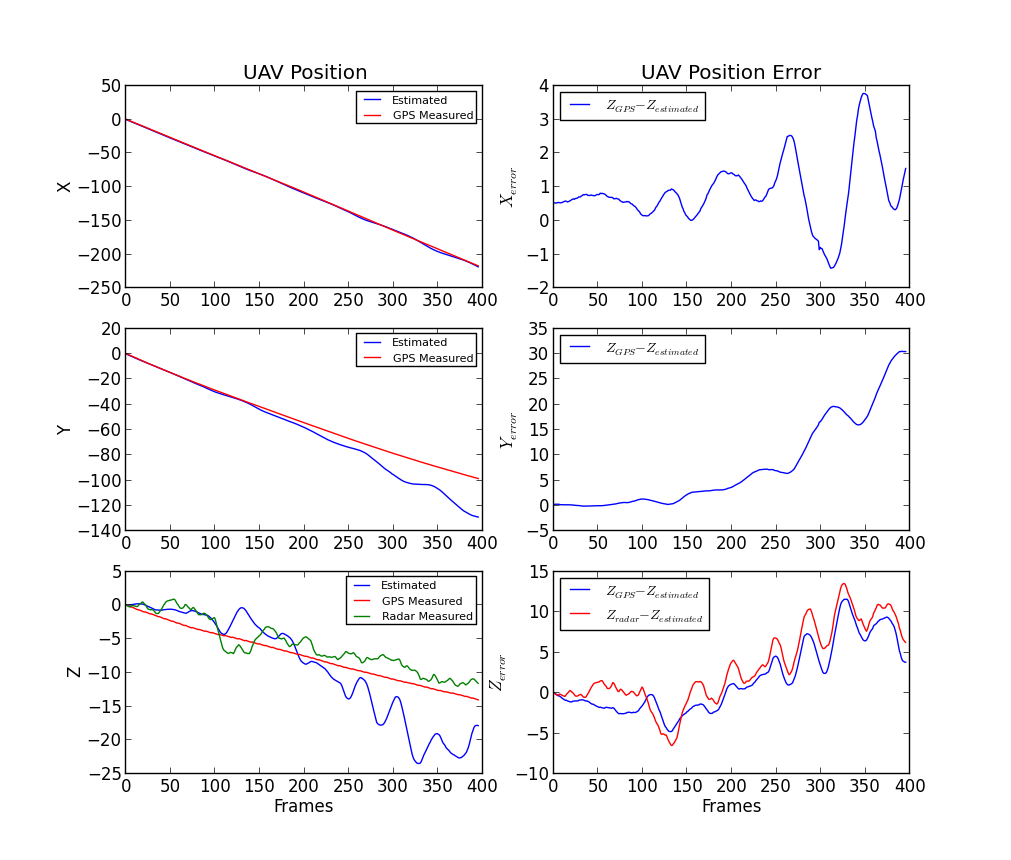
\includegraphics[width=13cm, keepaspectratio=true]
{./Figures/fltfig/airport/UAV_position_and_error.png}
\caption{SUAS position accuracy compared to GPS}
\label{fltfig:13}
\end{figure}

\begin{figure}[h]
\centering
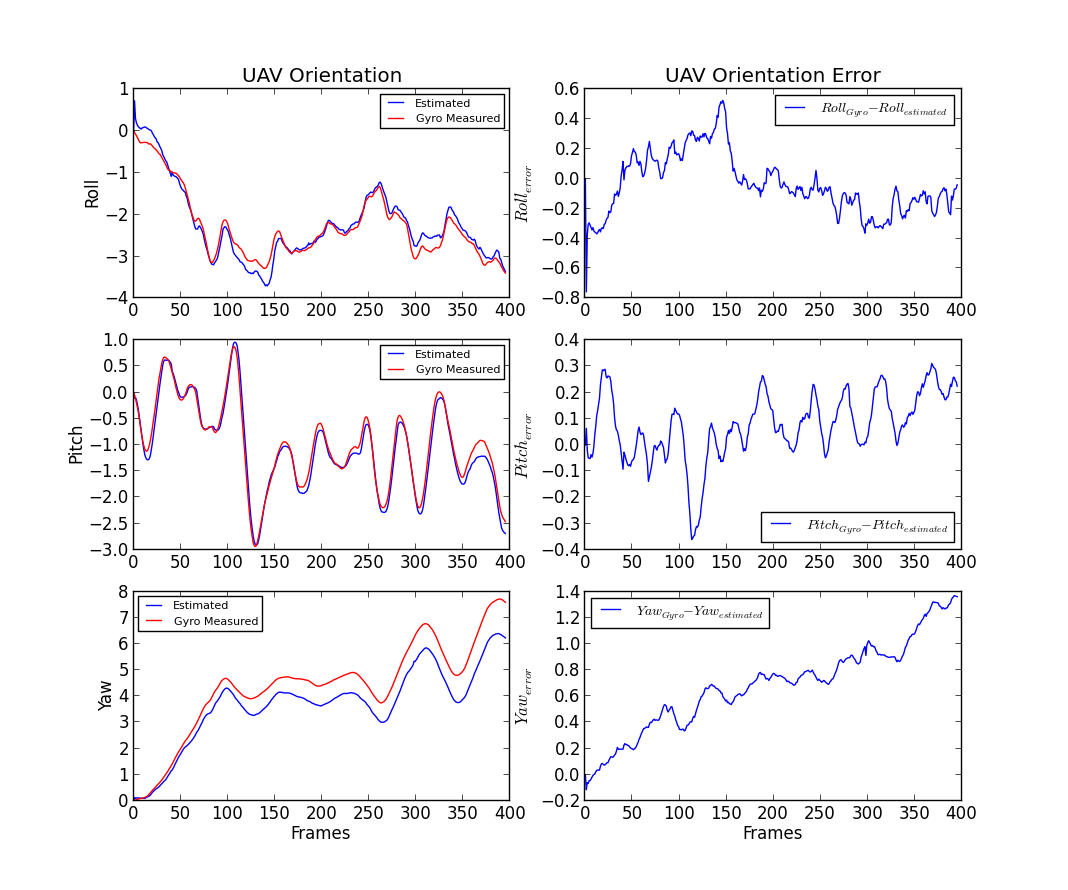
\includegraphics[width=13cm, keepaspectratio=true]
{./Figures/fltfig/airport/UAV_orientation_and_error.png}
\caption{SUAS orientation accuracy compared to magnetometer}
\label{fltfig:14}
\end{figure}
\FloatBarrier

Figure \ref{fltfig:15} shows the features positions in X and Y axis.
The google earth map provide very rough elevation data, therefore it
was not used. The ground truth X and Y coordinate of the features were
measured on Google Earth in GPS coordinates and converted into UTM.
This plot shows a clear offset error between the ground truth and the
estimated. X axis coordinate has a mean offset is about 100 meters,
and Y axis coordinate has a offset of about 130m. Since all features
are located in the bottom left corner of the FOV, it is more likely
for the lens distortion to be the main contributor to these error.


\begin{figure}[h]
\centering
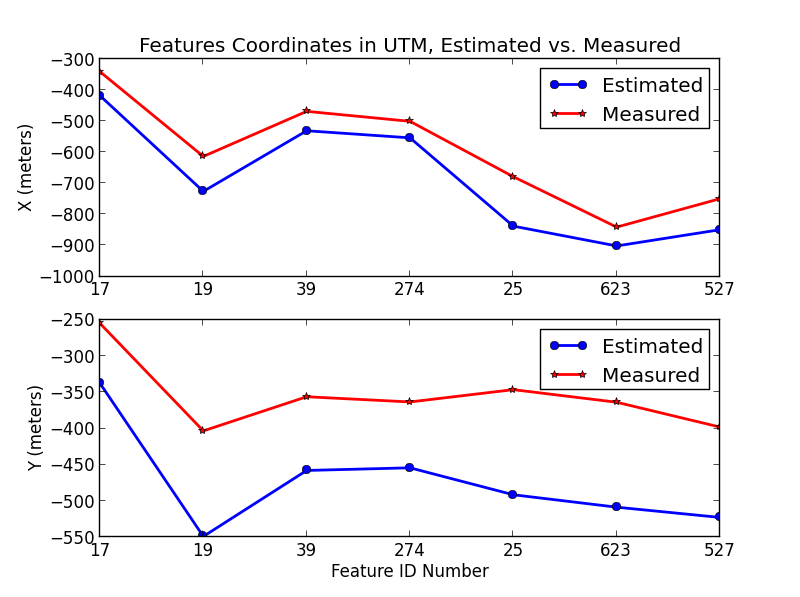
\includegraphics[width=13cm, keepaspectratio=true]
{./Figures/fltfig/airport/Feature_plot_(x,y).png}
\caption{Feature error on X and Y axis. }
\label{fltfig:15}
\end{figure}

%%% Local Variables:
%%% mode: latex
%%% TeX-master: "thesis"
%%% End:
